  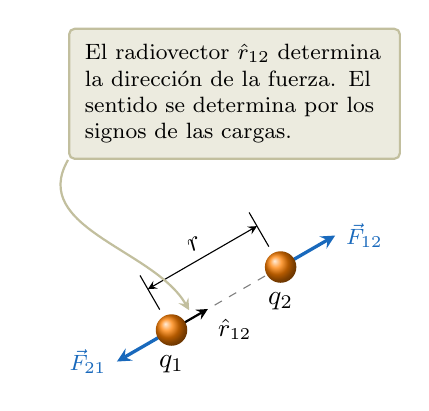
\begin{tikzpicture}[>=stealth]
    \def\h{.8}
    \def\l{1.6}
    \coordinate (r) at (30:\l/5);
    \draw[dashed,gray] (0,0) -- (30:\l);
    \draw[thin] (0,0) ++(120:.3) -- (120:\h); 
    \draw[thin] (30:\l) ++(120:.3) -- +(120:\h-.3);
    \draw[thin,<->] (120:.6) -- node[above,sloped] {$r$} +(30:\l);
    \draw[thick,->] (0,0) -- (30:\l/3) node[below right,font=\small] {$\hat{r}_{12}$};
    \draw[cyan!45!blue,->,very thick] (0,0) -- (210:\l/2) node[left,font=\footnotesize] {$\vec{F}_{21}$};
    \draw[cyan!45!blue,->,very thick] (30:\l) -- +(30:\l/2) node[right,font=\footnotesize] {$\vec{F}_{12}$};
    \shade[ball color=orange] (0,0) circle (.2) node[below=2mm] {$q_1$};
    \shade[ball color=orange] (30:\l) circle (.2) node[below=2mm] {$q_2$};
    
    \node (cartel) [
      font=\footnotesize,
      text width=3.8cm,
      align=left,
      fill=yellow!40!black!14,
      draw=yellow!40!black!46,
      thick,
      rounded corners=2pt,
      inner sep=2mm
      ]
      at (.8,3) {
        El radiovector $\hat{r}_{12}$ determina la dirección de la fuerza. El sentido se determina por los signos de las cargas.
    };

    \draw[->, thick, color=yellow!40!black!46, shorten >=3pt] 
             (cartel.south west) to[out=240, in=120] (r);
  \end{tikzpicture}
  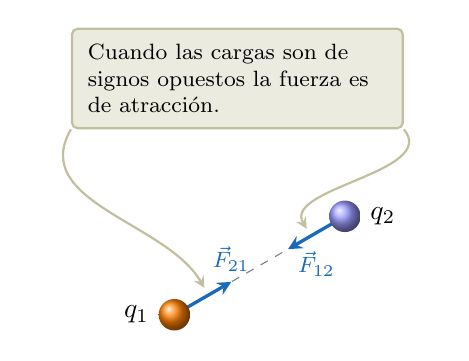
\begin{tikzpicture}[>=stealth]
    \def\h{.8}
    \def\l{2.5}
    \coordinate (r) at (30:\l/5);
    \draw[dashed,gray] (0,0) -- (30:\l);
    \draw[cyan!45!blue,->,very thick] (0,0) -- (30:\l/3) node[above,font=\footnotesize] {$\vec{F}_{21}$};
    \draw[cyan!45!blue,->,very thick] (30:\l) -- node[below=1mm,font=\footnotesize] {$\vec{F}_{12}$} +(210:\l/3);
    \shade[ball color=orange] (0,0) circle (.2) node[left=2mm] {$q_1$};
    \shade[ball color=blue!40] (30:\l) circle (.2) node[right=2mm] {$q_2$};
    
    \node (cartel) [
      font=\footnotesize,
      text width=3.8cm,
      align=left,
      fill=yellow!40!black!14,
      draw=yellow!40!black!46,
      thick,
      rounded corners=2pt,
      inner sep=2mm
      ]
      at (.8,3) {Cuando las cargas son de signos opuestos la fuerza es de atracción.};

    \draw[->, thick, color=yellow!40!black!46, shorten >=3pt] 
             (cartel.south west) to[out=240, in=120] (r);
    \draw[->, thick, color=yellow!40!black!46, shorten >=3pt] 
             (cartel.south east) to[out=310, in=120] (30:4*\l/5);
  \end{tikzpicture}
